\subsection{Panel specjalisty}

{\includegraphics{diagrams/use_cases/zobacz_panel_specjalisty.png}}

{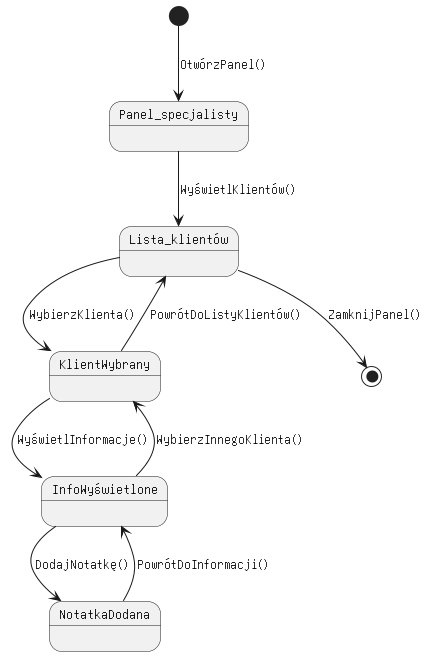
\includegraphics{diagrams/state/panel_specjalisty.png}}

\begin{enumerate}
\setcounter{enumi}{9}
\tightlist
\item
  {Zobacz panel specjalisty}
\end{enumerate}

{Aktorzy biorący udział: Specjalista (trener personalny, dietetyk,
fizjoterapeuta)}

{Cel przypadku: Wyświetlenie informacji dotyczących klientów specjalisty
i ich historii}

{Warunki początkowe: Specjalista jest zalogowany do systemu}

{Warunki końcowe: Specjalista widzi informacje dotyczące swoich klientów
i ich historii}

{Główny ciąg zdarzeń:}

\begin{enumerate}
\tightlist
\item
  {Specjalista loguje się do systemu.}
\item
  {Specjalista wybiera opcję "Panel specjalisty".}
\item
  {System wyświetla listę klientów przypisanych do specjalisty.}
\item
  {Specjalista wybiera jednego z klientów.}
\item
  {System wyświetla informacje dotyczące wybranego klienta, takie jak
  dane osobowe, historię treningów, dieta, rehabilitacja itp.}
\item
  {Specjalista może dodać notatki dotyczące wizyt i treningów klienta.}
\item
  {Specjalista kończy przeglądanie informacji i wylogowuje się z
  systemu.}
\end{enumerate}

{Alternatywne ciągi zdarzeń:}

\begin{itemize}
\tightlist
\item
  {W przypadku braku klientów przypisanych do specjalisty, system
  wyświetli stosowną informację.}
\end{itemize}